%************************
\subsection{Mischen von Modellen}
\label{sec:merging}

Das Mischen von Modellen unterscheidet sich vom Patchen unter anderem dadurch, dass die geänderten Modelle aus einem gleichen Basismodell entstanden sind.
Abbildung \ref{silift-tutorial_difference_merging} zeigt ein typisches Szenario des 3-Wege-Mischens.

\begin{figure}[H]
\centering
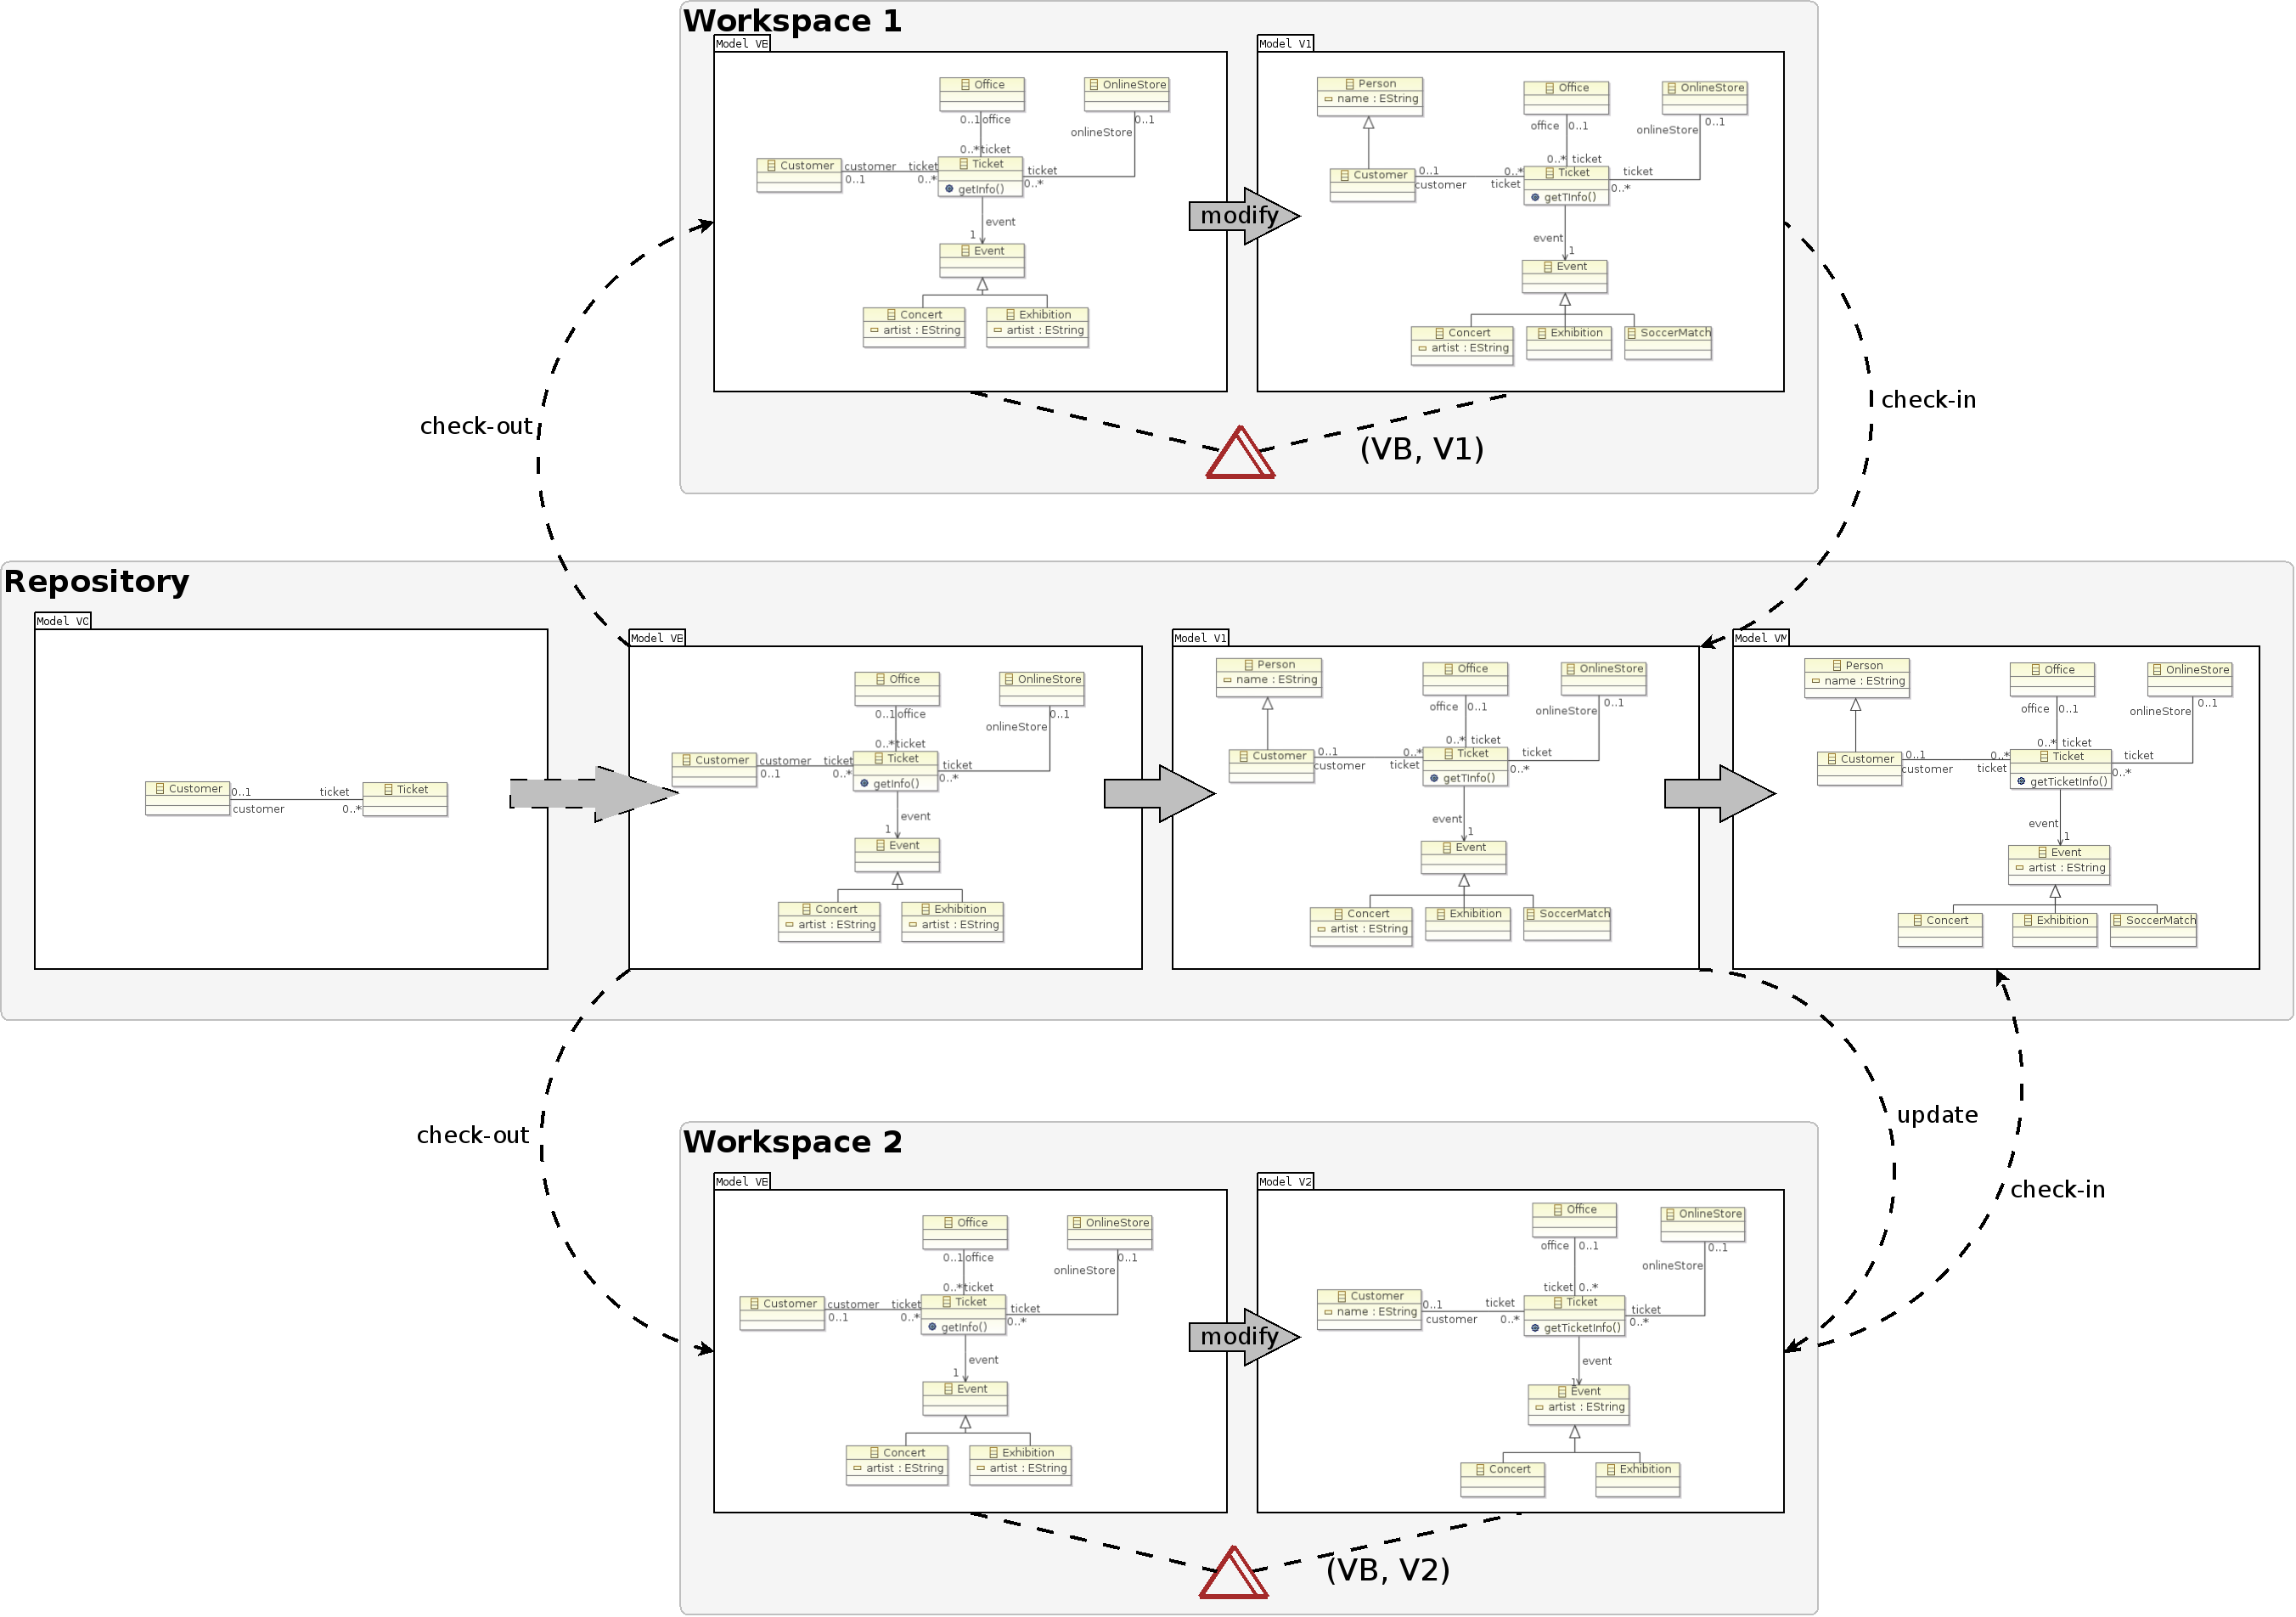
\includegraphics[width=\textwidth]{merging/graphics/silift-tutorial_difference_merging.png}
\caption{SiLift: Ablauf eines Mischvorganges}
\label{silift-tutorial_difference_merging}
\end{figure}

Jeder Workspace besitzt seine eigene Kopie des Basismodells (\texttt{Model VB}).
Diese werden unabhängig von einander modifiziert (\texttt{Model V1}, \texttt{Model V2}).
Nachdem die Änder\-ung\-en $\Delta(VB,V1)$ in \texttt{Workspace 1} abegschlossen sind, werden diese auf das Basismodell im \texttt{Repository} angewandt.
Da sich die Basisversion im \texttt{Repository} geändert hat, muss \texttt{Modell V2} in \texttt{Workspace 2} erst aktualisert, d.h. die Änderungen aus $\Delta(VB,V1)$ über\-nom\-men werden, bevor die Änderungen $\Delta(VB,V2)$ auf das Modell im \texttt{Repository} angewandt werden können.
Dabei kann es zu inkompatiblen bzw. unverträglichen Änderungen kommen, sogenannten Konflikten.
In diesem Szenario lassen sich drei solcher Konflikte ausmachen:
\begin{enumerate}[(1)]
	\item Konkurrierende Änderung der Operation \texttt{Ticket.getInfo()}.
	\item Redundante Erzeugung des Attributs \texttt{name}.
	\item Nicht einheitliche Definition des Attributs \texttt{artist}.
\end{enumerate}
Um die Konflikte zu lösen, muss man sich für eine der beiden Änderungen entscheiden, d.h. eine der Änderungen wird verworfen.
Eine weitere Möglichkeit besteht darin, beide Änderungen zu verwerfen und das Modell an der betroffenen Stelle manuell anzupassen.\\

Im Folgenden lernen Sie, wie Sie mit Hilfe von SiLift Modelle mischen können.

Selektieren Sie im Package- bzw. Project-Explorer das Basismodell, sowie die beiden geänderten Modelle und öffnen Sie mit der rechten Maustaste das Kontextmenü.
Wählen Sie \texttt{SiLift} $\triangleright$  \texttt{Three-Way-Merge} aus (vgl. Abb. \ref{silift-tutorial_merging_contextmenu}).

\begin{figure}[H]
\centering
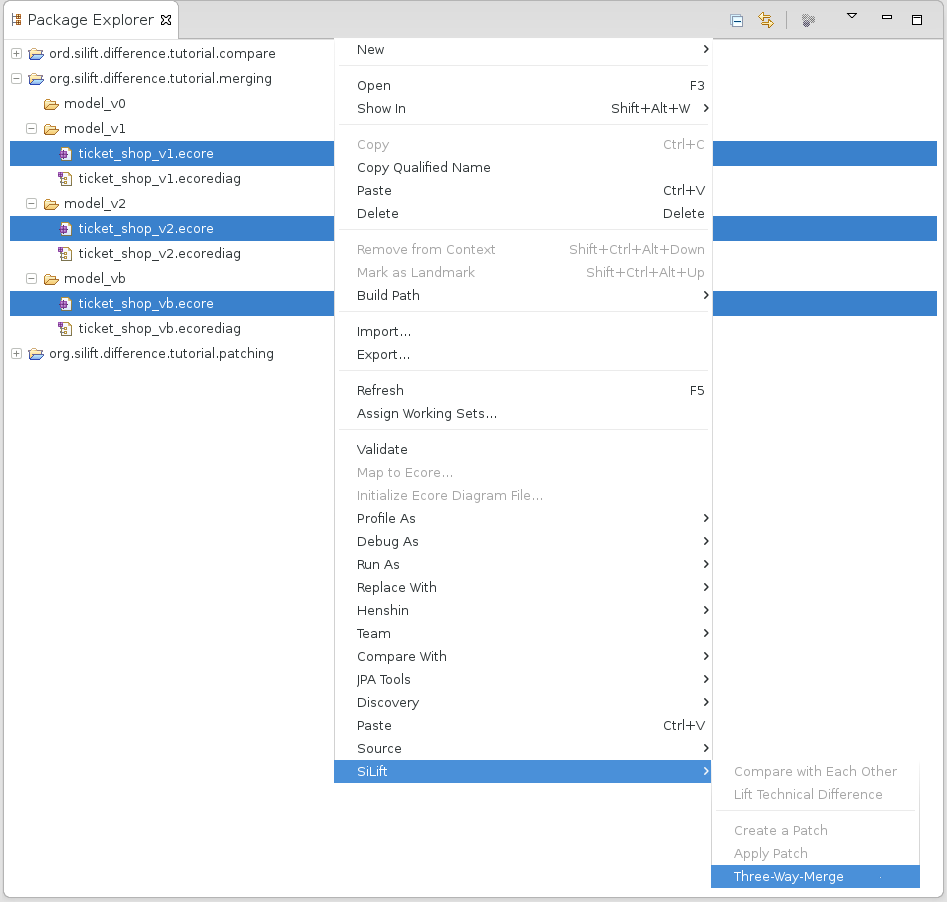
\includegraphics[width=0.8\textwidth]{merging/graphics/silift-tutorial_merging_contextmenu.png}
\caption{SiLift: 3-Wege-Mischen}
\label{silift-tutorial_merging_contextmenu}
\end{figure}

Es öffnet sich ein Konfigurationsdialog, der weitestgehend denen aus Abbildung \ref{silift-tutorial_patching_create_config}, \ref{silift-tutorial_patching_apply_config_page01} und \ref{silift-tutorial_patching_apply_config_page02} entspricht.
Die einzige Ausnahme ist, dass die Rolle der ausgewählten Modelle angegeben werden muss (vgl. Abb. \ref{silift-tutorial_merging_wizard}).

\begin{figure}[H]
\centering
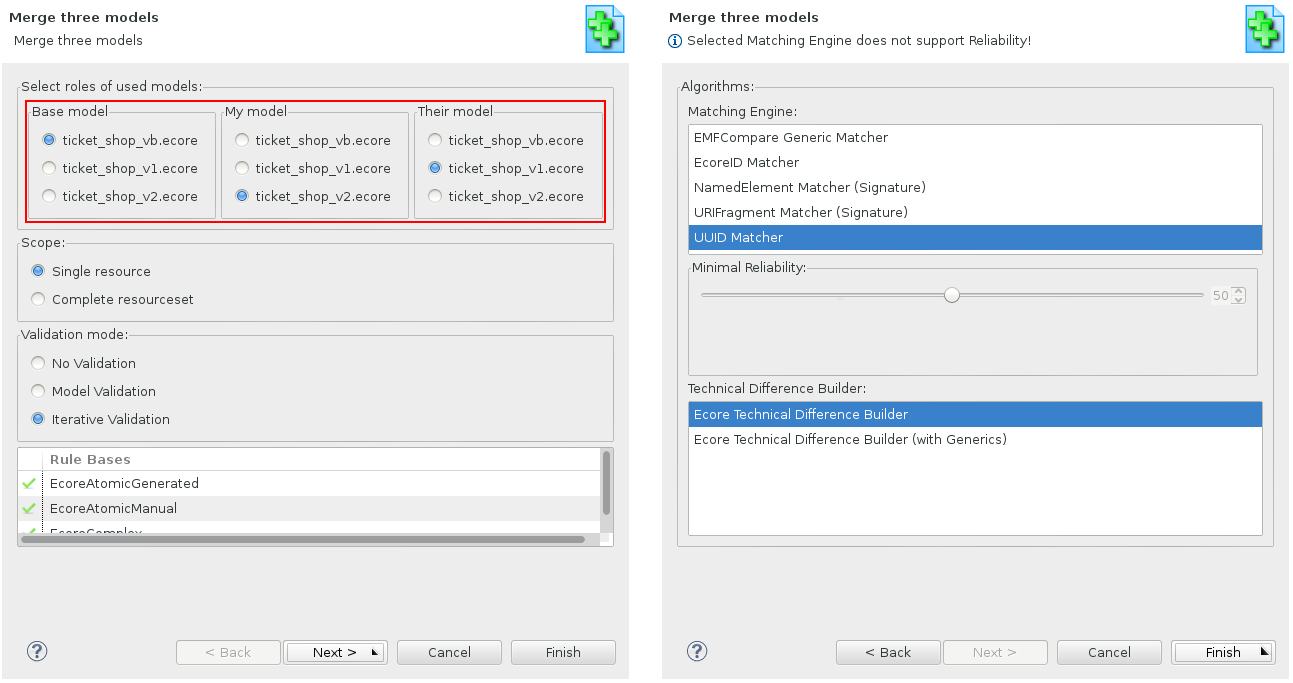
\includegraphics[width=0.8\textwidth]{merging/graphics/silift-tutorial_merging_wizard.png}
\caption{SiLift: Konfiguration des 3-Wege-Mischens}
\label{silift-tutorial_merging_wizard}
\end{figure}

Nachdem Sie auf \texttt{Finish} geklickt haben, öffnet sich die SiLift-Perspektive (vgl. Abb. \ref{silift-tutorial_merging_perspective}), welche bereits in Abschnitt \ref{sec:patching_apply} vorgestellt wurde.

\begin{figure}[H]
\centering
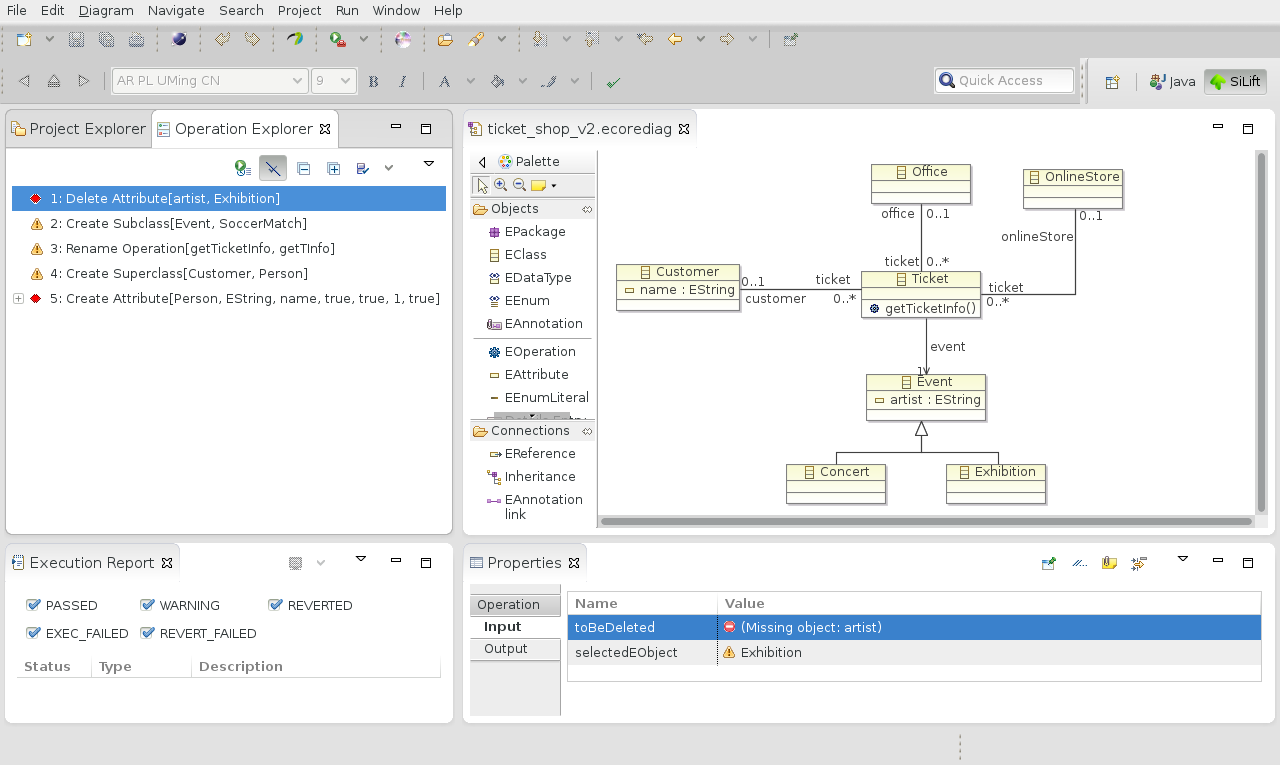
\includegraphics[width=0.8\textwidth]{merging/graphics/silift-tutorial_merging_perspective.png}
\caption{SiLift: 3-Wege-Mischen Perspektive}
\label{silift-tutorial_merging_perspective}
\end{figure}

Mit Hilfe des Operation-Explorer können nun analog zu Abschnitt \ref{sec:patching_apply} die Änderungen $\Delta(VB,V1)$ auf das eigene Modell angewandt werden.
Dabei werden konfliktbehaftete Operationen, deren Ausführung u.U. eigene Änderungen übschreiben, entsprechend ge\-kenn\-zeich\-net (vgl. Abb. \ref{silift-tutorial_merging_operation_explorer}).


\begin{figure}[H]
\centering
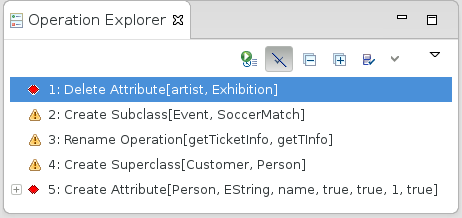
\includegraphics[width=0.6\textwidth]{merging/graphics/silift-tutorial_merging_operation_explorer.png}
\caption{SiLift: Operation Explorer}
\label{silift-tutorial_merging_operation_explorer}
\end{figure}

